% 第 21 题坐标图：按固定源 PDF 矢量路径换算（1 数学单位 = 85.0 pt → 2.988 cm；按比例作图）。
% 坐标原点即两轴交点；椭圆 C: x²+4y²=1（半轴 1.0/0.5，线宽 0.8）；抛物线 E: x²=2y 顶点在原点、
% 只画 x 轴以上部分（至 x=±1.2）；切线 l（斜率 0.5399）、线段 OM、过 P 的竖直线（上下均越出图形本体）、
% 线段 FP。图上无实心圆点、坐标轴无刻度。l 为斜置斜体字母。标注按源字形框中心定位（显式坐标）。
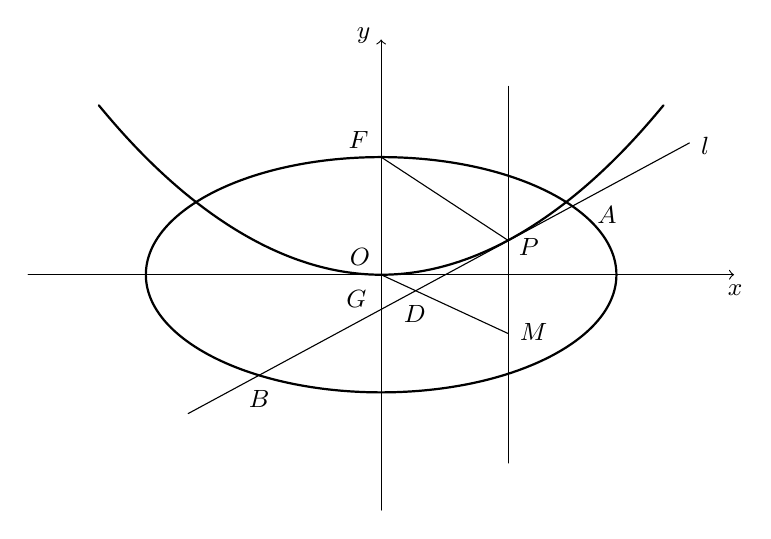
\begin{tikzpicture}[line cap=round,line join=round,font=\small,x=2.988cm,y=2.988cm]
% 坐标轴
\draw[->] (-1.50,0)--(1.50,0);
\draw[->] (0,-1.00)--(0,1.00);
% 椭圆（线宽 0.8，与源一致）与抛物线
\draw[line width=0.8pt] (0,0) ellipse (1.0 and 0.5);
\draw[line width=0.8pt] (-1.2,0.72) parabola bend (0,0) (1.2,0.72);
% 切线 l、线段 OM、过 P 的竖直线、线段 FP
\draw (-0.820,-0.590)--(1.310,0.560);
\draw (0,0)--(0.5399,-0.25);
\draw (0.5399,-0.80)--(0.5399,0.80);
\draw (0,0.5)--(0.5399,0.1458);
% ===== 标注（显式坐标，照源字形框中心）=====
\node[anchor=center,inner sep=0] at (-0.074,1.017) {\(y\)};
\node[anchor=center,inner sep=0] at (1.505,-0.066) {\(x\)};
\node[anchor=center,inner sep=0] at (-0.096,0.574) {\(F\)};
\node[anchor=center,inner sep=0] at (-0.0895,0.0741) {\(O\)};
% G 左上移（源位贴近切线，400 dpi 连通域实证并入；照清晰度优先原则微调）
\node[anchor=center,inner sep=0] at (-0.105,-0.105) {\(G\)};
\node[anchor=center,inner sep=0] at (0.6278,0.1184) {\(P\)};
\node[anchor=center,inner sep=0] at (0.6483,-0.2417) {\(M\)};
% A 右下移（源位贴近切线与椭圆，400 dpi 连通域实证并入；照清晰度优先原则微调至椭圆外）
\node[anchor=center,inner sep=0] at (0.96,0.252) {\(A\)};
\node[anchor=center,inner sep=0] at (0.143,-0.1675) {\(D\)};
\node[anchor=center,inner sep=0] at (-0.518,-0.5275) {\(B\)};
\node[anchor=center,inner sep=0] at (1.377,0.548) {\(l\)};
\end{tikzpicture}
